%%%%%%%%%%%%%%%%%%%%%%%%%%%%%%%%%%%%%%%%%
% Short Sectioned Assignment LaTeX Template Version 1.0 (5/5/12)
% This template has been downloaded from: http://www.LaTeXTemplates.com
% Original author:  Frits Wenneker (http://www.howtotex.com)
% License: CC BY-NC-SA 3.0 (http://creativecommons.org/licenses/by-nc-sa/3.0/)
%%%%%%%%%%%%%%%%%%%%%%%%%%%%%%%%%%%%%%%%%

%----------------------------------------------------------------------------------------
%	PACKAGES AND OTHER DOCUMENT CONFIGURATIONS
%----------------------------------------------------------------------------------------

\documentclass[paper=a4, fontsize=11pt]{scrartcl} % A4 paper and 11pt font size

% ---- Entrada y salida de texto -----

\usepackage[T1]{fontenc} % Use 8-bit encoding that has 256 glyphs
\usepackage[utf8]{inputenc}
%\usepackage{fourier} % Use the Adobe Utopia font for the document - comment this line to return to the LaTeX default

% ---- Idioma --------

\usepackage[spanish, es-tabla]{babel} % Selecciona el español para palabras introducidas automáticamente, p.ej. "septiembre" en la fecha y especifica que se use la palabra Tabla en vez de Cuadro

% ---- Otros paquetes ----

\usepackage{url} % ,href} %para incluir URLs e hipervínculos dentro del texto (aunque hay que instalar href)
\usepackage{hyperref}
\hypersetup{
	colorlinks=true,
	linkcolor=black,
	urlcolor=black,
	citecolor=black,
}
\usepackage{amsmath,amsfonts,amsthm} % Math packages
%\usepackage{graphics,graphicx, floatrow} %para incluir imágenes y notas en las imágenes
\usepackage{graphics,graphicx, float} %para incluir imágenes y colocarlas

% Para hacer tablas comlejas
%\usepackage{multirow}
%\usepackage{threeparttable}

%\usepackage{sectsty} % Allows customizing section commands
%\allsectionsfont{\centering \normalfont\scshape} % Make all sections centered, the default font and small caps

\usepackage{fancyhdr} % Custom headers and footers
\pagestyle{fancyplain} % Makes all pages in the document conform to the custom headers and footers
\fancyhead{} % No page header - if you want one, create it in the same way as the footers below
\fancyfoot[L]{} % Empty left footer
\fancyfoot[C]{} % Empty center footer
\fancyfoot[R]{\thepage} % Page numbering for right footer
\renewcommand{\headrulewidth}{0pt} % Remove header underlines
\renewcommand{\footrulewidth}{0pt} % Remove footer underlines
\setlength{\headheight}{13.6pt} % Customize the height of the header

\numberwithin{equation}{section} % Number equations within sections (i.e. 1.1, 1.2, 2.1, 2.2 instead of 1, 2, 3, 4)
\numberwithin{figure}{section} % Number figures within sections (i.e. 1.1, 1.2, 2.1, 2.2 instead of 1, 2, 3, 4)
\numberwithin{table}{section} % Number tables within sections (i.e. 1.1, 1.2, 2.1, 2.2 instead of 1, 2, 3, 4)

\setlength\parindent{0pt} % Removes all indentation from paragraphs - comment this line for an assignment with lots of text

\newcommand{\horrule}[1]{\rule{\linewidth}{#1}} % Create horizontal rule command with 1 argument of height
\usepackage{booktabs}

\usepackage{listings}
\lstdefinelanguage
[x64]{Assembler}     % add a "x64" dialect of Assembler
[x86masm]{Assembler} % based on the "x86masm" dialect
{morekeywords={CDQE,CQO,CMPSQ,CMPXCHG16B,JRCXZ,LODSQ,MOVSXD, %
		POPFQ,PUSHFQ,SCASQ,STOSQ,IRETQ,RDTSCP,SWAPGS, %
		rax,rdx,rcx,rbx,rsi,rdi,rsp,rbp, %
		r8,r8d,r8w,r8b,r9,r9d,r9w,r9b, %
		r10,r10d,r10w,r10b,r11,r11d,r11w,r11b, %
		r12,r12d,r12w,r12b,r13,r13d,r13w,r13b, %
		r14,r14d,r14w,r14b,r15,r15d,r15w,r15b}} % etc.
\usepackage{color}
\usepackage{xcolor}
\lstdefinestyle{customc}{
	belowcaptionskip=1\baselineskip,
	breaklines=true,
	frame=L,
	xleftmargin=\parindent,
	language=C,
	showstringspaces=false,
	basicstyle=\footnotesize\ttfamily,
	keywordstyle=\bfseries\color{green!40!black},
	commentstyle=\itshape\color{purple!40!black},
	identifierstyle=\color{blue},
	stringstyle=\color{orange},
}

\lstset{escapechar=@,style=customc}
\usepackage{url}


\title{	
	\normalfont \normalsize
	\begin{figure}[htb]
		\centering
		
\includegraphics[width=0.3\textwidth]{./imagenes/1}
	\end{figure}
	\textsc{\textbf{Estructura de Computadores} \\ Grado en Ingeniería Informática \\ 
	Curso 2018-2019} \\ [25pt] % Your university, school and/or department name(s)
	\begin{figure}[htb]
		\centering
		
\includegraphics[width=0.15\textwidth]{./imagenes/2}
	\end{figure}
	\horrule{0.5pt} \\[0.4cm] % Thin top horizontal rule
	\huge Memoria Práctica 4. \\
	\huge Bomba Digital - Desensambladores.
	\\ % The assignment title
	\horrule{2pt} \\[0.5cm] % Thick bottom horizontal rule
}
\author{Félix Ramírez García  \\
\href{mailto:felixramirezgarcia@correo.ugr.es}{felixramirezgarcia@correo.ugr.es}} % Nombre y apellidos
\date{\normalsize\today} % Incluye la fecha actual

%----------------------------------------------------------------------------------------
% DOCUMENTO
%----------------------------------------------------------------------------------------

\begin{document}
	
	\maketitle % Muestra el Título
	
	\newpage %inserta un salto de página
	
	\tableofcontents % para generar el índice de contenidos
	
	\listoffigures % para generar índice de imágenes.
	
	\listoftables % para generar índice de tablas.
	
	\newpage
	
	
	%-----------------------------------------------------------------------
	%						Programar la bomba digital
	%-----------------------------------------------------------------------
	\section[4.1-Programar la bomba digital]{4.1-Programar la bomba digital}
	
	A continuación se va a explicar como desactivar mi bomba paso a paso, para ello abrimos el ejecutable con gdb ,
	usamos layout asm y layout regs para activar el entorno gráfico , ponemos un breakpoint en main y ejecutamos. \\
	
	\begin{tabular}{c | c | c | c | c}
		\toprule
		Nombre Algoritmo &  N Clusters &     HC metric &  SC metric &        Time \\
		\midrule
		K-means          &           4 &  29697.858169 &   0.764292 &    0.100956 \\
		Birch            &           6 &  21480.901579 &   0.729611 &    0.646720 \\
		Ward             &          10 &  33361.232561 &   0.845975 &   19.899369 \\
		MeanShift        &          14 &  32215.188490 &   0.855566 &    0.784660 \\
		Spectral         &           3 &  26907.715611 &   0.726861 &  421.776694 \\
		Birch\_modificado &           4 &  14704.418333 &   0.669432 &    0.687701 \\
		Ward\_modificado  &          35 &  87235.116033 &   0.955259 &   11.627957 \\
		\bottomrule
	\end{tabular}
	
	\vspace{0.1in}
	
	Vamos avanzando con nexti hasta que nos solicite la contraseña, le introducimos una al azar y seguimos avanzando hasta que nos encontramos
	con la llamada a la función password\_chars . Usamos el comando stepi para entrar a la función cuyo código es el que muestra la figura 1.1 .
	
	\begin{figure}[htb]
		\centering
		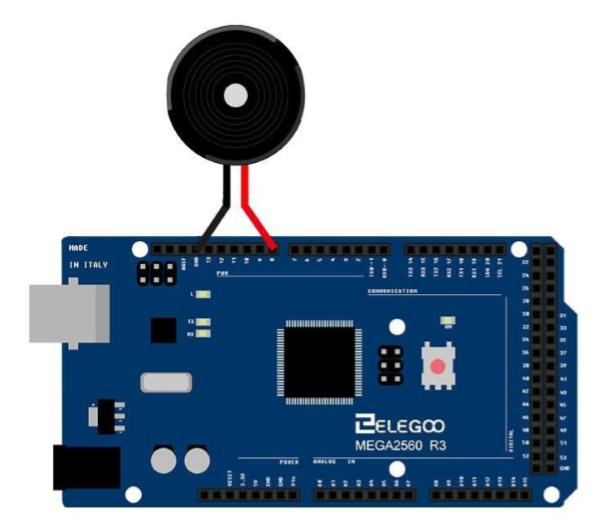
\includegraphics[width=0.6\textwidth]{./imagenes/3}
		\caption{.} \label{fig:1}
	\end{figure}
	
	
	Mientras seguimos avanzando nos damos cuenta de que la palabra que hemos introducido se guarda en rdi
	,y lo primero que hace es comparar la primera posición de la palabra 
	con la letra 'e' , y si esto es cierto realiza un cambio entre las posiciones 7 y 4 de la palabra . 
	En caso de que no se cumpla la condición de que la primera posición sea una 'e' se realiza un salto a password\_chars+127 , 
	instrucción que pone un uno en eax , condición para que explote la bomba.
	El código en ensamblador de esta parte de la función es que muestra la figura 1.2 .  
	
	\begin{figure}[htb]
		\centering
		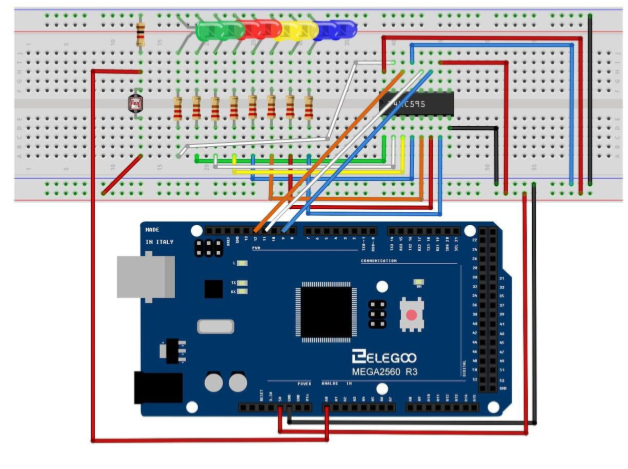
\includegraphics[width=0.7\textwidth]{./imagenes/4}
		\caption{Primer swap de chars de la funcion password char..} \label{fig:1}
	\end{figure}
	
	Mientras seguimos avanzando nos damos cuenta de que esta misma estructura se repite dos veces mas , una segunda comprobando si la tercera posición de la palabra es la letra 'o' , y si lo es, cambia las letras de las posiciones 8 y 1 .
	En caso de que no se cumpla la condición de que la tercera posición sea una 'o' se realiza un salto a password\_chars+134 , 
	instrucción que aumenta en uno el valor de eax , condición para que explote la bomba.
	El código de esta segunda parte es el muestra la figura 1.3
	
	\begin{figure}[htb]
		\centering
		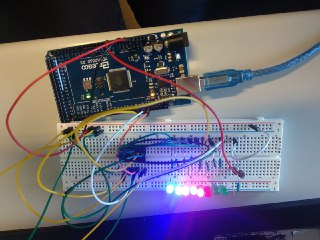
\includegraphics[width=0.7\textwidth]{./imagenes/5}
		\caption{Segundo swap de chars de la funcion password char..} \label{fig:1}
	\end{figure}
	
	En la tercera vez que se repite esta estructura se compara la séptima posición de la palabra con la letra 'l' , y en caso de que lo sea se realiza un 
	cambio de letras entre las posiciones 4 y 0 de la palabra.
	En caso de que no se cumpla la condición de que la séptima posición sea una 'l' se realiza un salto a password\_chars+139 , 
	instrucción que aumenta en uno el valor de eax , condición para que explote la bomba.
	El código de esta tercera parte es el que muestra la figura 1.4. \\
	
	\begin{figure}[htb]
		\centering
		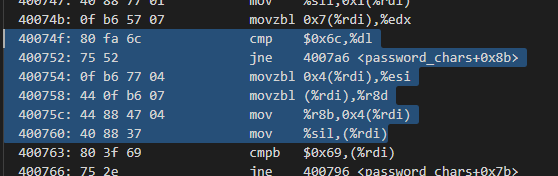
\includegraphics[width=0.7\textwidth]{./imagenes/6}
		\caption{Tercer swap de chars de la funcion password char.} \label{fig:1}
	\end{figure}	 
	
	Por lo tanto ya tenemos que la primera posición (Empezando a contar por el 0) de la palabra tiene la letra 'e' , la tercera posición de la palabra tiene la 'o',	y la séptima posición tiene la 'l' . Para pasar esta fase hay que introducir una palabra con la primera letra una 'e' , la tercera letra una 'o' , y en la cuarta letra una 'l' (Porque se cambia en el primer swap con la posición 7). \\
	
	Al seguir avanzando , nos encontramos con nueve comprobaciones mas , las que muestra la figura 1.5 .
	
	\begin{figure}[htb]
		\centering
		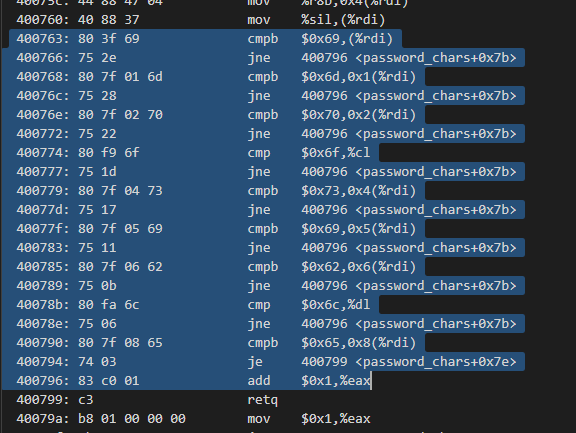
\includegraphics[width=0.8\textwidth]{./imagenes/7}
		\caption{Comprobaciones finales de password char.} \label{fig:1}
	\end{figure}
	
	Si cualquiera de estas nueve comparaciones falla, se saltaría a password\_chars+126 , instrucción que aumenta en uno el valor de eax , condición para que explote la bomba. \\
	
	La primera condición comprueba si la letra en la posición numero cero es la 'i' (0x69), la segunda condición comprueba si la letra en la posición numero uno es la 'm' (0x6d), la tercera condición comprueba si la letra en la posición numero dos es la 'p' (0x70), la cuarta condición comprueba si la letra en la posición numero tres es la 'o' (0x6f), la quinta condición comprueba si la letra en la posición numero cuatro es la 's' (0x73), la sexta condición comprueba si la letra en la posición numero cinco es la 'i' (0x69), la séptima condición comprueba si la letra en la posición numero seis es la 'b' (0x62), la octava condición comprueba si la letra en la posición numero siete es la 'l' (0x6c) y la novena condición comprueba si la letra en la posición numero ocho es la 'e' (0x65) . \\
	
	A partir de aquí se puede deducir que la palabra encriptada es 'imposible' y ahora tenemos que recorrer de forma inversa la función   para simular el proceso de encriptacion del final a principio. Por lo tanto tenemos que recorrer los tres condicionales comentados anteriormente para saber cual es la palabra sin encriptar. \\
	
	Partiendo ahora de la palabra 'imposible' , vamos a aplicarle el tercer condicional , que cambia las posiciones 0 y 4 . Ahora tenemos la palabra 
	'smpoiible' . Después le aplicamos el segundo condicional , que cambia las letras de las posiciones 8 y 1 , quedándose la palabra en 'sepoiiblm' . Por último le aplicamos el cambio que realiza el primer condicional que nos encontramos al entrar en la función , el que intercambia las posiciones 7 y 4, quedándose la palabra resultado en 'sepolibim'. Para una comprensión mas clara de esta ultima parte esta la figura 1.6 . \\
	
	\begin{figure}[htb]
		\centering
		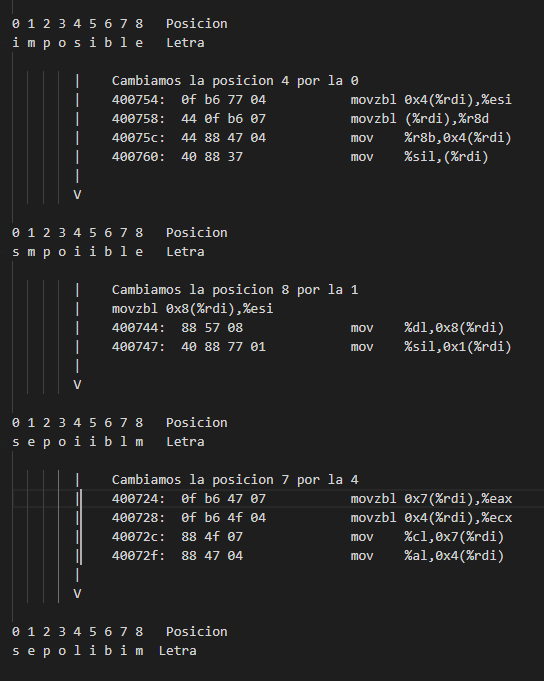
\includegraphics[width=0.5\textwidth]{./imagenes/8}
		\caption{Etapas de desencriptado.} \label{fig:1}
	\end{figure}
	
	Una vez tenemos la palabra y no nos explota la bomba en esta función podemos seguir avanzando hasta encontrarnos con la llamada a la segunda función , password\_number .Introducimos algo al azar y una vez dentro con stepi podemos ver en su código que almacena el numero en el registro edi, el código es el que muestra la figura 1.7 .
	
	\begin{figure}[htb]
		\centering
		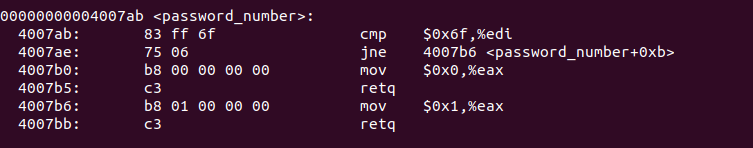
\includegraphics[width=0.7\textwidth]{./imagenes/9}
		\caption{Funcion password number.} \label{fig:1}
	\end{figure}
	
	Aquí simplemente se hace una comprobación con 0x6f , y si es correcta , la función devuelve un 0 , condición para desactivar la bomba. 
	Por lo tanto esta contraseña no es mas que el numero 0x6f en decimal . El numero 111 .   \\
	
	Una vez sabemos todo esto se puede ejecutar el programa con las contraseñas 'sepolibim' y '111' y desactivar la bomba . Ahora vamos a modificar 
	ambas contraseñas del ejecutable , para ello vamos a sustituir la letra p de la contraseña 'sepolivim' por una v . Esto lo hacemos abriendo el ejecutable
	con ghex y buscando la secuencia en hexadecimal que realiza la función password\_chars para la comprobación de la palabra almacenada en la posición numero dos (Empezando por la cero) de rdi .La figura 1.8 muestra la búsqueda de la secuencia en hexadecimal '80 7f 02 70'.
	
	\begin{figure}[htb]
		\centering
		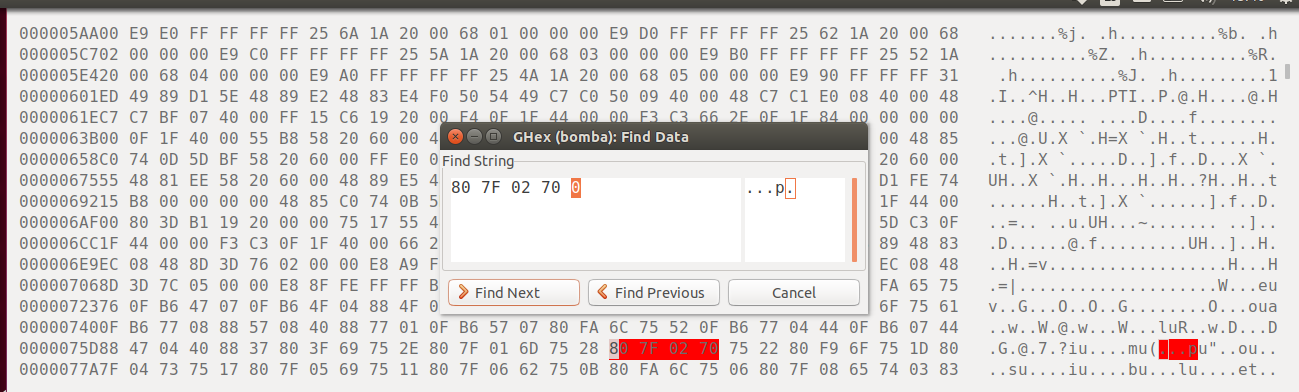
\includegraphics[width=0.9\textwidth]{./imagenes/10}
		\caption{Busqueda de la comprobacion de la palabra para la letra p y sustitucion por la v} \label{fig:1}
	\end{figure}
	
	Como se puede apreciar en la figura ,el par de dígitos que representa a la letra p es el '70' , por lo que si los sustituimos por 76 habremos cambiado la palabra 'sepolibim' por 'sevolibim'. \\
	
	Por último vamos a modificar la contraseña numérica , para ello buscamos en ghex la secuencia en hexadecimal que hace la comprobación con el numero 11 , la secuencia '83 ff 6f' , y modificamos el valor de 6f por el de 7f , cambio que muestra la figura 1.9 . Quedando ahora la contraseña numérica en 127.
	
	\begin{figure}[htb]
		\centering
		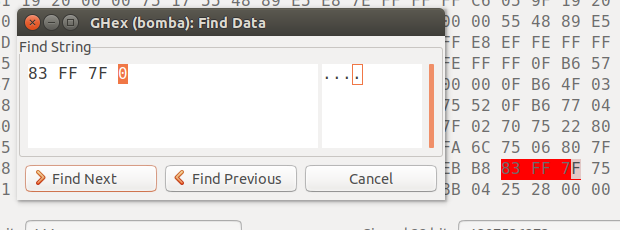
\includegraphics[width=0.9\textwidth]{./imagenes/11}
		\caption{Busqueda de la comprobacion del numero 111 y sustitucion por el 127} \label{fig:1}
	\end{figure}
	
	Para concluir esta sección se van a mostrar en la figura 1.10 la ejecución de ambas bombas , una primera sin modificaciones , y una segunda alterada .\\
	
	\begin{figure}[htb]
		\centering
		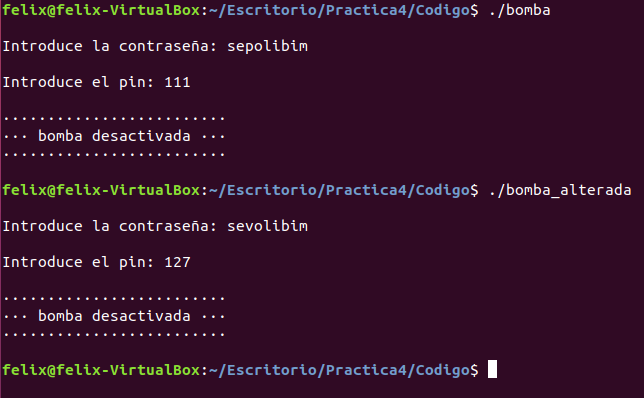
\includegraphics[width=0.7\textwidth]{./imagenes/12}
		\caption{Ejecucion de ambas bombas} \label{fig:1}
	\end{figure}
	
	\vspace{0.06in}
	
	\begin{tabular}{c | c | c | c | c}
		\toprule
		{} &  N Clusters &    HC metric &  SC metric &      Time \\
		\midrule
		K-means              &          10 &  6943.576223 &   0.679065 &  0.045921 \\
		Birch                &          10 &  4081.202946 &   0.697422 &  0.043426 \\
		Ward                 &          15 &  7978.888763 &   0.696960 &  0.173204 \\
		MeanShift            &           9 &  3675.392770 &   0.714534 &  0.059399 \\
		Spectral             &           5 &  6059.545108 &   0.706452 &  1.043716 \\
		Birch\_modificado     &           5 &  2615.276048 &   0.690900 &  0.042927 \\
		meanshift\_modificado &          10 &  3757.968423 &   0.715982 &  0.056404 \\
		\bottomrule
	\end{tabular}
	
	\vspace{0.06in}
		
	%-----------------------------------------------------------------------
	%							BIBLIOGRAFIA
	%-----------------------------------------------------------------------
	% Referencia a bibliografia			En \cite{Baz}
	% Referencia a figura				La figura (\ref{fig:1})
	% Espacio entre lineas				\vspace{0.06in}
	% Figura con comentario al pie
	%\begin{figure}[htb]
	%	\centering
	%	
\includegraphics[width=0.4\textwidth]{./imagenes/1}
	%	\caption{Universidad de Granada.} \label{fig:1}
	%\end{figure}
	%\begin{thebibliography}{99}
	%	\bibitem{Baz} 
	%	\textsc{Bazaraa, M.S., J.J. Jarvis}
	%	\textit{Programacuib}.
	%	\newline
	%	\url{https://www.google.es}	
	%\end{thebibliography}

	


\end{document}